% !TEX program = xelatex
\documentclass[11pt,a4paper]{article}

% Minimalist Vietnamese LaTeX report
\usepackage[a4paper,margin=2.2cm]{geometry}
\usepackage{fontspec}
\setmainfont{TeX Gyre Termes}
\setsansfont{TeX Gyre Heros}
\setmonofont{DejaVu Sans Mono}

\usepackage{microtype}
\usepackage{amsmath,amssymb}
\usepackage{booktabs,longtable,tabularx,array}
\usepackage{enumitem}
\usepackage{xcolor}
\usepackage{hyperref}
\usepackage{titlesec}
\usepackage{fancyhdr}
\usepackage{pgfplots}
\usepackage{pdflscape}
\pgfplotsset{compat=1.18}

\definecolor{ink}{HTML}{1F2937}
\definecolor{muted}{HTML}{6B7280}
\definecolor{linegray}{HTML}{E5E7EB}

\hypersetup{
    colorlinks=true,
    linkcolor=ink,
    urlcolor=ink,
    citecolor=ink
}

\setlength{\parindent}{0pt}
\setlength{\parskip}{6pt}
\renewcommand{\arraystretch}{1.12}
\pagestyle{fancy}
\fancyhf{}
\lhead{\small Online Caching + ML}
\rhead{\small \thepage}
\renewcommand{\headrulewidth}{0.3pt}

\titleformat{\section}{\Large\bfseries\sffamily\color{ink}}{\thesection}{0.7em}{}
\titleformat{\subsection}{\large\bfseries\sffamily\color{ink}}{\thesubsection}{0.7em}{}
\titleformat{\subsubsection}{\normalsize\bfseries\sffamily\color{ink}}{\thesubsubsection}{0.7em}{}

\newcommand{\code}[1]{\texttt{#1}}
\newcommand{\hedge}{\code{HedgeFullDelayedAllExpertSoft}}
\newcommand{\rawml}{\code{RawML}}
\newcommand{\mr}{\mathrm{MR}}

\begin{document}

\begin{titlepage}
    \centering
    \vspace*{2.5cm}
    {\Huge\bfseries\sffamily Online Caching tăng cường Machine Learning\\[0.25cm]
    bằng HedgeFullDelayedAllExpertSoft\par}
    \vspace{0.8cm}
    {\large Báo cáo dự án tối giản dựa trên dữ liệu trong thư mục \code{data/processed}\par}
    \vspace{1.5cm}
    \begin{tabular}{rl}
        \textbf{Bài toán:} & Online cache replacement / online decision-making \\
        \textbf{Nhánh ML phụ trợ:} & Supervised regression dự đoán khoảng cách truy cập tiếp theo \\
        \textbf{Thuật toán chính:} & \hedge{} với các expert LRU, LFU, MARK, RawML \\
        \textbf{Bộ dữ liệu:} & 13 trace Chledowski benchmark \\
        \textbf{Ngày lập báo cáo:} & \today
    \end{tabular}

    \vfill
    {\small Repository: \code{tin03092006-cell/Online-Caching}}
\end{titlepage}

\section*{Tóm tắt điều hành}

Dự án giải quyết bài toán \textbf{online caching}: tại mỗi thời điểm, hệ thống nhận một request mới và phải quyết định giữ hoặc loại bỏ phần tử nào khỏi cache khi cache đã đầy, trong khi không biết toàn bộ chuỗi request tương lai. Mục tiêu thực nghiệm là giảm số lần cache miss so với các chính sách cổ điển như LRU, LFU và MARK, đồng thời so sánh khoảng cách với Belady/OPT, thuật toán tối ưu ngoại tuyến chỉ dùng làm mốc lý tưởng. Phương pháp chính là \hedge{}, một cơ chế online learning kết hợp bốn expert: LRU, LFU, MARK và \rawml{}. Trong đó \rawml{} là mô hình Gradient Boosting Regressor học từ các đặc trưng thời gian truy cập như recency, frequency, recent frequency, average inter-arrival và cache age để dự đoán \code{target\_next\_distance}. Trên 13 dataset benchmark, toàn bộ pipeline chạy thành công, không có dataset lỗi. Tổng số request test là 1,173,888. Kết quả cho thấy \hedge{} đạt 1,035,223 cache misses, thấp hơn MARK khoảng 6.98\%, thấp hơn LFU khoảng 2.36\% và thấp hơn LRU khoảng 6.88\%. Tuy nhiên, thuật toán vẫn còn cách Belady/OPT khoảng 9.39\% theo tổng số miss, cho thấy còn dư địa cải thiện mô hình dự đoán và chiến lược gán trọng số expert.

\tableofcontents
\newpage

\section{Giới thiệu bài toán}

\subsection{Phát biểu bài toán}

Bài toán cốt lõi của dự án là \textbf{online cache replacement}. Cho một chuỗi request
\[
    r_1, r_2, \ldots, r_T,
\]
và một cache có sức chứa tối đa \(k\) item. Tại thời điểm \(t\), nếu \(r_t\) đã nằm trong cache thì xảy ra cache hit. Nếu \(r_t\) chưa nằm trong cache thì xảy ra cache miss; nếu cache đã đầy, thuật toán phải chọn một item đang nằm trong cache để evict trước khi đưa \(r_t\) vào cache.

Đây \textbf{không phải} là bài toán phân loại, hồi quy hay phân cụm thuần túy. Bài toán tổng thể là một bài toán \textbf{ra quyết định online}. Tuy vậy, trong pipeline có một bài toán học máy con thuộc dạng \textbf{hồi quy}: dự đoán \code{target\_next\_distance}, tức khoảng cách từ thời điểm hiện tại đến lần truy cập tiếp theo của một item. Nếu dự đoán item nào còn rất lâu mới được truy cập lại, thuật toán có thể ưu tiên evict item đó.

\subsection{Động lực}

Caching xuất hiện trong hệ điều hành, cơ sở dữ liệu, trình duyệt, CDN, hệ thống lưu trữ, bộ nhớ đệm CPU và nhiều hệ thống phục vụ request quy mô lớn. Cache miss thường đắt hơn cache hit vì hệ thống phải truy cập bộ nhớ chậm hơn, ổ đĩa, mạng hoặc tầng lưu trữ phía sau. Do đó, giảm cache miss giúp giảm độ trễ, giảm tải hệ thống và tăng hiệu suất tài nguyên.

Các thuật toán cổ điển như LRU, LFU và MARK đơn giản, dễ triển khai, nhưng thường chỉ dựa trên lịch sử gần hoặc tần suất quá khứ. Trong nhiều trace thực tế, quy luật truy cập có thể thay đổi theo thời gian. Vì vậy, cách tiếp cận trong dự án là kết hợp nhiều expert bằng online learning: khi một expert hoạt động tốt trên đoạn trace hiện tại, trọng số của expert đó tăng tương đối; khi hoạt động kém, trọng số giảm.

\subsection{Mục tiêu}

Dự án đặt ra ba mục tiêu cụ thể:

\begin{enumerate}[leftmargin=1.4em]
    \item Xây dựng pipeline benchmark chạy được local, miễn phí, không yêu cầu GPU.
    \item Đánh giá thuật toán \hedge{} trên 13 trace benchmark, so sánh với Belady/OPT, MARK, LRU và LFU.
    \item Đạt tổng số cache misses thấp hơn MARK, LRU và LFU trên toàn bộ tập test; đồng thời phân tích rõ các trace mà thuật toán thắng, hòa hoặc thua.
\end{enumerate}

\section{Mô tả và khám phá dữ liệu}

\subsection{Nguồn dữ liệu}

Dữ liệu sử dụng trong báo cáo nằm trong thư mục \code{data/processed}. Ba file quan trọng là:

\begin{itemize}[leftmargin=1.4em]
    \item \code{chledowski\_trace\_report.csv}: thống kê quá trình chuẩn hóa trace, số request, số item unique và cache size được chọn.
    \item \code{summary\_all\_datasets\_with\_lru\_lfu.csv}: kết quả benchmark sau khi bổ sung LRU và LFU.
    \item \code{RUN\_REPORT.md}: báo cáo chạy tự động, metadata, kết quả từng dataset và trạng thái thành công/thất bại.
\end{itemize}

Pipeline benchmark dùng 13 dataset: \code{astar}, \code{bwaves}, \code{cactusadm}, \code{gems}, \code{lbm}, \code{leslie3d}, \code{libq}, \code{mcf}, \code{omnetpp}, \code{sphinx3}, \code{xalanc}, \code{bzip}, \code{milc}. Tất cả dataset đều chạy thành công; không có dataset thất bại. Tổng số request test là 1,173,888.

\subsection{Kích thước dữ liệu}

\begin{longtable}{lrrrrr}
\caption{Kích thước các trace sau khi chuẩn hóa.}\\
\toprule
Dataset & Train req. & Valid req. & Test req. & Unique test & Cache size \\
\midrule
\endfirsthead
\toprule
Dataset & Train req. & Valid req. & Test req. & Unique test & Cache size \\
\midrule
\endhead
astar & 1,154,048 & 144,256 & 144,256 & 520 & 51 \\
bwaves & 570,368 & 71,296 & 71,296 & 21,751 & 512 \\
cactusadm & 221,952 & 27,744 & 27,744 & 13,532 & 512 \\
gems & 723,456 & 90,432 & 90,432 & 44,037 & 512 \\
lbm & 782,080 & 97,760 & 97,760 & 76,982 & 512 \\
leslie3d & 716,032 & 89,504 & 89,504 & 4,350 & 434 \\
libq & 579,840 & 72,480 & 72,480 & 1,638 & 163 \\
mcf & 2,965,504 & 370,688 & 370,688 & 86,118 & 512 \\
omnetpp & 555,520 & 69,440 & 69,440 & 2,338 & 233 \\
sphinx3 & 328,704 & 41,088 & 41,088 & 653 & 65 \\
xalanc & 69,120 & 8,640 & 8,640 & 2,419 & 241 \\
bzip & 167,680 & 20,960 & 20,960 & 3,554 & 355 \\
milc & 556,800 & 69,600 & 69,600 & 25,860 & 512 \\
\bottomrule
\end{longtable}

\subsection{Đặc trưng và biến mục tiêu}

Từ mỗi trạng thái cache, pipeline tạo các đặc trưng số cho từng item đang nằm trong cache:

\begin{tabularx}{\textwidth}{lX}
\toprule
Đặc trưng & Ý nghĩa \\
\midrule
\code{recency} & Khoảng cách từ lần truy cập gần nhất đến thời điểm hiện tại. \\
\code{frequency} & Tổng số lần item đã được truy cập trong quá khứ. \\
\code{recent\_frequency} & Số lần item xuất hiện trong cửa sổ truy cập gần đây. \\
\code{average\_inter\_arrival} & Khoảng cách trung bình giữa hai lần truy cập liên tiếp của item. \\
\code{cache\_age} & Thời gian item đã nằm trong cache kể từ lúc được đưa vào. \\
\code{target\_next\_distance} & Biến mục tiêu: khoảng cách đến lần truy cập tiếp theo của item. \\
\bottomrule
\end{tabularx}

Về mặt ra quyết định, nếu một item có \code{target\_next\_distance} càng lớn thì item đó càng phù hợp để bị evict. Belady/OPT dùng đúng thông tin tương lai này nên chỉ là oracle ngoại tuyến. \rawml{} cố gắng học xấp xỉ đại lượng đó từ lịch sử.

\subsection{EDA: insight quan trọng}

\subsubsection{Độ khó của dữ liệu}

Một chỉ báo độ khó là tỉ lệ
\[
    \frac{\text{unique items trong test}}{\text{cache size}}.
\]
Nhiều dataset có số item unique lớn hơn cache size hàng chục đến hàng trăm lần. Ví dụ, \code{mcf} có 86,118 unique item trong test nhưng cache size chỉ là 512, tức tỉ lệ khoảng 168.2. \code{lbm} có tỉ lệ khoảng 150.4. Những trace này tạo áp lực rất lớn lên thuật toán vì cache không thể giữ được phần lớn không gian item.

Tuy vậy, tỉ lệ unique/cache không phải yếu tố duy nhất quyết định miss ratio. \code{mcf} rất khó theo số lượng item, nhưng \hedge{} vẫn cải thiện mạnh so với MARK. Điều này cho thấy trace \code{mcf} có cấu trúc truy cập mà LFU hoặc ML có thể khai thác tốt hơn MARK thuần túy.

\subsubsection{Tương quan ở mức trace}

Vì file tổng hợp hiện tại lưu kết quả benchmark và thống kê trace, không lưu toàn bộ ma trận đặc trưng từng dòng, correlation matrix dưới đây được tính ở mức trace, không phải ở mức từng sample huấn luyện.

\begin{center}
\begin{tabular}{lrrr}
\toprule
Biến & Unique/cache & Hedge MR & Hedge improv. \\
\midrule
Unique/cache & 1.000 & -0.398 & 0.574 \\
Hedge MR & -0.398 & 1.000 & -0.837 \\
Hedge improv. & 0.574 & -0.837 & 1.000 \\
\bottomrule
\end{tabular}
\end{center}

Diễn giải: trên 13 trace, improvement của \hedge{} so với MARK có tương quan dương vừa phải với tỉ lệ unique/cache. Tuy nhiên, số mẫu chỉ là 13 nên đây chỉ là insight khám phá, không phải bằng chứng nhân quả. Tương quan âm mạnh giữa Hedge miss ratio và Hedge improvement là hợp lý: khi thuật toán giảm được miss ratio, improvement so với MARK thường tăng.

\subsubsection{Outliers}

Các outlier đáng chú ý:

\begin{itemize}[leftmargin=1.4em]
    \item \code{mcf}: số request test lớn nhất, số unique test rất lớn, nhưng \hedge{} cải thiện 22.80\% so với MARK.
    \item \code{lbm}: Belady/OPT, LRU, LFU, MARK và \hedge{} đều có miss ratio bằng 1.0. Điều này cho thấy trace gần như không tạo cơ hội tái sử dụng trong điều kiện cache size hiện tại.
    \item \code{libq}: validation MAE rất thấp, nhưng miss ratio vẫn gần 1.0. Điều này cho thấy MAE của mô hình dự đoán chưa đủ để kết luận thuật toán cache sẽ tốt; quyết định eviction còn phụ thuộc vào cấu trúc request và lựa chọn expert.
    \item \code{bzip}: \hedge{} chỉ thua MARK đúng 1 cache miss, nên đây không phải thất bại lớn về mặt thực nghiệm.
\end{itemize}

\section{Tiền xử lý dữ liệu}

\subsection{Làm sạch dữ liệu}

Script benchmark tự động dò định dạng file, xác định cột item request, trích xuất chuỗi request và ghi về dạng mỗi dòng một item. Các file được nhận diện chủ yếu là \code{two\_columns\_no\_header}; cột item được chọn là cột thứ hai. Báo cáo trace cho thấy số dòng bị bỏ qua bằng 0 trên tất cả dataset, vì vậy không có bằng chứng về missing values hoặc dòng rác sau bước parse.

\subsection{Chia tập dữ liệu}

Benchmark sử dụng ba phần: train, validation và test. Trong cấu hình tự động, \code{benchmark\_chledowski.py} có tham số mặc định \code{train\_ratio = 0.8}, \code{validation\_ratio = 0.1}; phần còn lại là test. Nếu dataset có sẵn file train/valid/test thì script dùng các file đó; nếu không, script nối trace rồi chia theo tỉ lệ.

Train dùng để học mô hình \rawml{}. Validation dùng để chọn learning rate cho Hedge. Test dùng để báo cáo kết quả cuối cùng.

\subsection{Feature engineering}

Feature engineering là phần quan trọng của dự án. Thay vì đưa trực tiếp item ID vào mô hình, hệ thống tạo các biến động theo thời gian:

\[
    x_i(t) =
    \left[
    \text{recency},
    \text{frequency},
    \text{recent\_frequency},
    \text{average\_inter\_arrival},
    \text{cache\_age}
    \right].
\]

Các biến này có ý nghĩa trực tiếp với caching:

\begin{itemize}[leftmargin=1.4em]
    \item \code{recency} giúp mô phỏng trực giác của LRU.
    \item \code{frequency} và \code{recent\_frequency} giúp mô phỏng trực giác của LFU nhưng linh hoạt hơn.
    \item \code{average\_inter\_arrival} mô tả chu kỳ truy cập.
    \item \code{cache\_age} mô tả thời gian item đã chiếm tài nguyên cache.
\end{itemize}

\subsection{Encoding và scaling}

Item ID không được one-hot encoding, vì số lượng item unique có thể rất lớn và one-hot sẽ gây sparse vector kích thước cao. Thay vào đó, mô hình chỉ dùng các đặc trưng số đã nêu. Mô hình \rawml{} là Gradient Boosting Regressor, nên không bắt buộc phải dùng StandardScaler hoặc MinMaxScaler như SVM hay neural network. Đây là lựa chọn hợp lý cho bài toán local vì gradient boosting chạy được CPU và xử lý feature scale không đồng nhất khá tốt.

\section{Phương pháp luận và mô hình}

\subsection{Các baseline}

Báo cáo dùng năm nhóm thuật toán:

\begin{tabularx}{\textwidth}{lX}
\toprule
Thuật toán & Vai trò \\
\midrule
Belady/OPT & Oracle ngoại tuyến, biết tương lai, dùng làm mốc lý tưởng thấp nhất về cache miss. \\
LRU & Baseline cổ điển, evict item ít được truy cập gần đây nhất. \\
LFU & Baseline cổ điển, evict item có tần suất truy cập thấp nhất trong cache. \\
MARK & Baseline randomized online có nền tảng competitive analysis. \\
\hedge{} & Thuật toán đề xuất, kết hợp LRU, LFU, MARK và \rawml{} bằng online learning. \\
\bottomrule
\end{tabularx}

\subsection{Mô hình RawML}

\rawml{} dùng \code{GradientBoostingRegressor} với cấu hình:

\begin{itemize}[leftmargin=1.4em]
    \item \code{learning\_rate = 0.05}
    \item \code{n\_estimators = 100}
    \item \code{max\_depth = 3}
    \item \code{max\_training\_rows = 50000}
\end{itemize}

Đầu vào là các đặc trưng cache-level ở từng thời điểm. Đầu ra là dự đoán khoảng cách truy cập tiếp theo. Khi cần evict, \rawml{} chọn item có khoảng cách dự đoán lớn nhất.

\subsection{Thuật toán HedgeFullDelayedAllExpertSoft}

\hedge{} không tin tuyệt đối vào một expert. Tại mỗi cache miss khi cache đầy:

\begin{enumerate}[leftmargin=1.4em]
    \item LRU, LFU, MARK và \rawml{} cùng đề xuất item nên evict.
    \item Hedge dùng trọng số hiện tại của các expert để tổng hợp phiếu.
    \item Item có điểm tổng hợp cao nhất bị evict.
    \item Feedback không đến ngay lập tức. Nếu item từng được một expert đề xuất evict xuất hiện lại trong tương lai, expert đó nhận loss phụ thuộc vào độ trễ feedback:
    \[
        \ell = \frac{1}{1 + \Delta t}.
    \]
    \item Trọng số expert được cập nhật theo dạng mũ:
    \[
        w_i \leftarrow w_i \exp(-\eta \ell_i).
    \]
\end{enumerate}

Phiên bản \code{AllExpertSoft} còn giữ lại vai trò của các expert cổ điển làm anchor. Điều này giúp thuật toán không bị phụ thuộc hoàn toàn vào \rawml{} khi dự đoán ML nhiễu hoặc không ổn định.

\subsection{Độ đo đánh giá}

Các độ đo chính:

\[
    \mr = \frac{\text{cache misses}}{\text{total requests}}.
\]

\[
    \rho_A = \frac{\text{misses của thuật toán } A}{\text{misses của Belady/OPT}}.
\]

\[
    \text{Improvement vs MARK}
    =
    \frac{\text{MARK misses} - \text{Algorithm misses}}
    {\text{MARK misses}}
    \times 100\%.
\]

Cache miss là độ đo quan trọng nhất vì nó đo trực tiếp chi phí vận hành của hệ thống cache. MAE của \rawml{} chỉ là độ đo phụ để đánh giá mô hình dự đoán khoảng cách truy cập; MAE tốt không nhất thiết kéo theo cache miss thấp, vì quyết định eviction còn phụ thuộc vào tương tác giữa nhiều expert.

\section{Thực nghiệm và kết quả}

\subsection{Chiến lược huấn luyện}

Với mỗi dataset, pipeline thực hiện:

\begin{enumerate}[leftmargin=1.4em]
    \item Chuẩn hóa trace về chuỗi item request.
    \item Chọn cache size theo luật \code{ratio}: cache size bằng khoảng 1\% số unique item, bị chặn bởi \code{min\_cache\_size = 16} và \code{max\_cache\_size = 512}.
    \item Tạo training frame từ train trace.
    \item Huấn luyện \rawml{}.
    \item Chọn \(\eta\) cho Hedge trên validation trace từ tập ứng viên \(\{0.1, 0.3, 0.7, 1.0\}\).
    \item Chạy Belady/OPT, LRU, LFU, MARK và \hedge{} trên test trace.
\end{enumerate}

\subsection{Tổng hợp kết quả}

\begin{center}
\begin{tabular}{lrrrr}
\toprule
Thuật toán & Total misses & Weighted MR & Avg. MR & Avg. comp. ratio \\
\midrule
Belady/OPT & 946,386 & 0.8062 & 0.8312 & 1.0000 \\
\hedge{} & 1,035,223 & 0.8819 & 0.9367 & 1.1602 \\
LFU & 1,060,265 & 0.9032 & 0.9612 & 1.2000 \\
LRU & 1,111,660 & 0.9470 & 0.9640 & 1.2027 \\
MARK & 1,112,906 & 0.9481 & 0.9623 & 1.1999 \\
\bottomrule
\end{tabular}
\end{center}

Theo tổng số cache misses trên toàn bộ test, \hedge{} là thuật toán online tốt nhất trong các thuật toán đã thử. Nó giảm:

\begin{itemize}[leftmargin=1.4em]
    \item 6.98\% tổng miss so với MARK.
    \item 6.88\% tổng miss so với LRU.
    \item 2.36\% tổng miss so với LFU.
\end{itemize}

Khoảng cách với Belady/OPT vẫn còn rõ: tổng miss của \hedge{} bằng khoảng 1.0939 lần Belady/OPT. Đây là kết quả hợp lý vì Belady/OPT biết toàn bộ tương lai, còn \hedge{} chỉ ra quyết định online.

\subsection{Biểu đồ tổng hợp}

\begin{center}
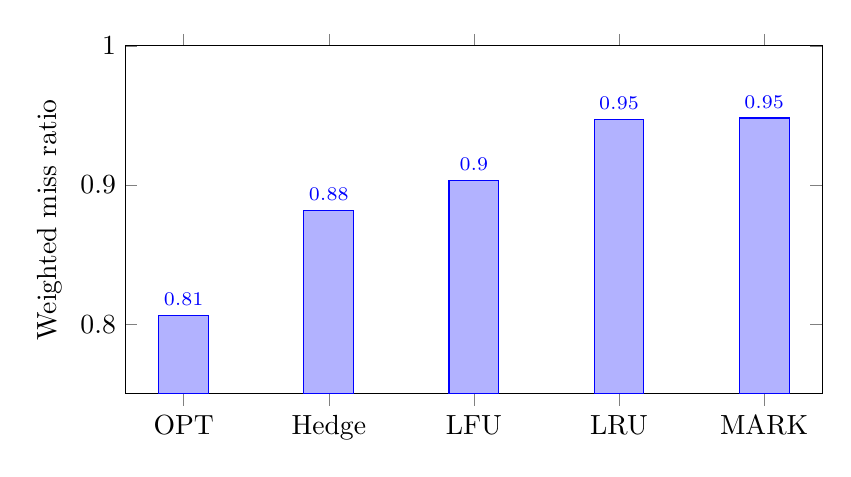
\begin{tikzpicture}
\begin{axis}[
    ybar,
    width=0.86\textwidth,
    height=6cm,
    ylabel={Weighted miss ratio},
    symbolic x coords={OPT,Hedge,LFU,LRU,MARK},
    xtick=data,
    ymin=0.75,
    ymax=1.0,
    bar width=18pt,
    nodes near coords,
    nodes near coords align={vertical},
    every node near coord/.append style={font=\scriptsize},
]
\addplot coordinates {(OPT,0.8062) (Hedge,0.8819) (LFU,0.9032) (LRU,0.9470) (MARK,0.9481)};
\end{axis}
\end{tikzpicture}
\end{center}

\subsection{Kết quả chi tiết theo dataset}

\begin{landscape}
\begin{longtable}{lrrrrrrr}
\caption{Miss ratio theo dataset. Cột cuối là improvement của \hedge{} so với MARK.}\\
\toprule
Dataset & Cache & OPT & MARK & LRU & LFU & Hedge & Improv. \\
\midrule
\endfirsthead
\toprule
Dataset & Cache & OPT & MARK & LRU & LFU & Hedge & Improv. \\
\midrule
\endhead
astar & 51 & 0.9721 & 0.9999 & 0.9999 & 0.9974 & 0.9999 & 0.00\% \\
bwaves & 512 & 0.9514 & 1.0000 & 1.0000 & 1.0000 & 1.0000 & 0.00\% \\
cactusadm & 512 & 0.7858 & 1.0000 & 1.0000 & 1.0000 & 0.9292 & 7.08\% \\
gems & 512 & 0.9007 & 0.9754 & 0.9746 & 0.9937 & 0.9741 & 0.13\% \\
lbm & 512 & 1.0000 & 1.0000 & 1.0000 & 1.0000 & 1.0000 & 0.00\% \\
leslie3d & 434 & 0.7998 & 0.9445 & 0.9406 & 0.9792 & 0.9328 & 1.24\% \\
libq & 163 & 0.9911 & 1.0000 & 1.0000 & 1.0000 & 1.0000 & 0.00\% \\
mcf & 512 & 0.5837 & 0.8696 & 0.8662 & 0.7099 & 0.6713 & 22.80\% \\
omnetpp & 233 & 0.7938 & 0.9868 & 0.9896 & 0.9840 & 0.9879 & -0.11\% \\
sphinx3 & 65 & 0.9190 & 1.0000 & 1.0000 & 1.0000 & 0.9793 & 2.06\% \\
xalanc & 241 & 0.6365 & 0.9147 & 0.9390 & 0.8888 & 0.8839 & 3.37\% \\
bzip & 355 & 0.4794 & 0.8185 & 0.8219 & 0.9426 & 0.8185 & -0.01\% \\
milc & 512 & 0.9927 & 1.0000 & 1.0000 & 1.0000 & 1.0000 & 0.00\% \\
\bottomrule
\end{longtable}
\end{landscape}

\subsection{Thắng, hòa, thua}

So với MARK, \hedge{}:

\begin{itemize}[leftmargin=1.4em]
    \item Thắng 7 dataset: \code{astar}, \code{cactusadm}, \code{gems}, \code{leslie3d}, \code{mcf}, \code{sphinx3}, \code{xalanc}.
    \item Hòa 4 dataset: \code{bwaves}, \code{lbm}, \code{libq}, \code{milc}.
    \item Thua 2 dataset: \code{omnetpp}, \code{bzip}.
\end{itemize}

Nếu tính best online theo từng dataset và cho phép hòa, \hedge{} nằm trong nhóm tốt nhất ở 10/13 dataset. Hai điểm sáng nhất là \code{mcf} và \code{xalanc}. Trên \code{mcf}, \hedge{} giảm miss so với MARK 22.80\% và còn tốt hơn cả LFU. Trên \code{xalanc}, \hedge{} đạt miss ratio 0.8839, tốt hơn MARK, LRU và LFU.

\section{Thảo luận và phân tích lỗi}

\subsection{Phân tích lỗi}

Hai dataset mà \hedge{} thua MARK là \code{omnetpp} và \code{bzip}. Trên \code{omnetpp}, \hedge{} có 68,599 misses còn MARK có 68,525 misses, tức thua 74 misses. Trên \code{bzip}, \hedge{} có 17,156 misses còn MARK có 17,155 misses, tức thua đúng 1 miss.

Có ba nguyên nhân hợp lý:

\begin{enumerate}[leftmargin=1.4em]
    \item \textbf{Feedback bị trễ}: loss chỉ được quan sát khi item bị evict xuất hiện lại. Nếu trace có pha truy cập ngắn hoặc chuyển pha nhanh, trọng số expert có thể cập nhật chậm.
    \item \textbf{RawML không luôn hữu ích}: mô hình hồi quy có thể có MAE thấp trên validation nhưng vẫn không chọn đúng item nên evict tại các thời điểm quan trọng.
    \item \textbf{Anchor chưa đủ thích nghi}: LRU/LFU là anchor tốt trong nhiều trace, nhưng nếu trace có cấu trúc phù hợp với MARK randomized hơn, việc pha trộn expert có thể gây nhiễu nhẹ.
\end{enumerate}

\subsection{Tầm quan trọng của đặc trưng}

Báo cáo benchmark hiện tại chưa lưu trực tiếp \code{feature\_importances\_} của Gradient Boosting Regressor, nên không nên bịa ra thứ hạng định lượng. Tuy nhiên, xét theo cơ chế cache, các đặc trưng có vai trò như sau:

\begin{itemize}[leftmargin=1.4em]
    \item \code{recency}: thường quan trọng vì nó là tín hiệu chính của locality theo thời gian.
    \item \code{frequency} và \code{recent\_frequency}: quan trọng khi trace có item phổ biến lặp lại nhiều lần.
    \item \code{average\_inter\_arrival}: hữu ích nếu item có chu kỳ truy cập tương đối đều.
    \item \code{cache\_age}: giúp phát hiện item nằm lâu trong cache nhưng không được truy cập lại.
\end{itemize}

Để làm phần feature importance chặt chẽ hơn, nên sửa pipeline để lưu thêm:
\[
    \code{predictor.model.feature\_importances\_}
\]
cho từng dataset sau khi train xong \rawml{}.

\subsection{Hạn chế}

Các hạn chế chính của dự án:

\begin{itemize}[leftmargin=1.4em]
    \item Cache size đang dùng luật 1\% số unique item và bị chặn tối đa 512; kết quả có thể thay đổi nếu dùng cache size khác.
    \item Chỉ dùng một seed là 42, trong khi MARK và Hedge có thành phần randomized.
    \item Mô hình ML hiện tại là Gradient Boosting Regressor đơn giản; chưa thử mô hình tuần tự như RNN/Transformer hoặc mô hình học theo phiên truy cập.
    \item Báo cáo hiện tại có EDA ở mức trace và kết quả benchmark; chưa lưu toàn bộ feature frame để phân tích correlation matrix ở mức sample.
    \item Belady/OPT chỉ là mốc ngoại tuyến, không thể triển khai thực tế vì cần biết tương lai.
\end{itemize}

\section{Kết luận và hướng phát triển}

\subsection{Kết luận}

Dự án đã giải quyết đúng bài toán đặt ra: xây dựng một pipeline online caching có yếu tố machine learning, chạy được local, đánh giá trên nhiều trace và so sánh với các baseline quan trọng. Kết quả tổng hợp cho thấy \hedge{} là thuật toán online tốt nhất trong nhóm đã thử, với tổng số cache misses thấp hơn MARK, LRU và LFU. Đặc biệt, trên \code{mcf}, thuật toán cải thiện rất mạnh so với MARK và vượt cả LFU, cho thấy việc kết hợp online learning với expert ML là có giá trị.

Tuy nhiên, kết quả cũng cho thấy không thể khẳng định thuật toán thắng tuyệt đối trên mọi trace. \hedge{} vẫn thua nhẹ trên \code{omnetpp} và \code{bzip}, và còn cách Belady/OPT. Vì vậy, đóng góp chính của dự án nên được trình bày là: \textbf{một thuật toán online caching kết hợp nhiều expert, đạt kết quả tổng thể tốt hơn các baseline online trong benchmark hiện tại}, chứ không phải một thuật toán tối ưu tuyệt đối.

\subsection{Hướng phát triển}

Các hướng cải thiện tiếp theo:

\begin{enumerate}[leftmargin=1.4em]
    \item Chạy nhiều cache size khác nhau, ví dụ 0.5\%, 1\%, 2\%, 5\% số unique item.
    \item Chạy nhiều seed để đánh giá độ ổn định của MARK và Hedge.
    \item Lưu feature importance và prediction error theo từng dataset.
    \item Thử thêm expert mới như ARC, CLOCK, SIEVE hoặc một expert dựa trên mô hình tuần tự.
    \item Tách rõ benchmark ``online không dự đoán'', ``online có ML'', và ``offline oracle'' để báo cáo khoa học hơn.
    \item Đưa thuật toán vào một demo nhỏ: nhập trace, chọn cache size, xuất miss ratio và biểu đồ so sánh.
\end{enumerate}

\section{Tài liệu tham khảo}

\begin{thebibliography}{9}

\bibitem{belady1966}
L. A. Belady.
\newblock A study of replacement algorithms for a virtual-storage computer.
\newblock \emph{IBM Systems Journal}, 1966.

\bibitem{sleator1985}
D. D. Sleator and R. E. Tarjan.
\newblock Amortized efficiency of list update and paging rules.
\newblock \emph{Communications of the ACM}, 1985.

\bibitem{fiat1991}
A. Fiat, R. Karp, M. Luby, L. McGeoch, D. Sleator, and N. Young.
\newblock Competitive paging algorithms.
\newblock \emph{Journal of Algorithms}, 1991.

\bibitem{freund1997}
Y. Freund and R. E. Schapire.
\newblock A decision-theoretic generalization of on-line learning and an application to boosting.
\newblock \emph{Journal of Computer and System Sciences}, 1997.

\bibitem{sklearn}
Scikit-learn Developers.
\newblock \emph{GradientBoostingRegressor documentation}.
\newblock \url{https://scikit-learn.org/stable/modules/generated/sklearn.ensemble.GradientBoostingRegressor.html}

\bibitem{repo}
Repository nội bộ.
\newblock \emph{tin03092006-cell/Online-Caching}: các file \code{src/data.py}, \code{src/model.py}, \code{src/soft\_classic\_anchor.py}, \code{scripts/benchmark\_chledowski.py}, \code{data/processed/RUN\_REPORT.md} và \code{data/processed/summary\_all\_datasets\_with\_lru\_lfu.csv}.

\end{thebibliography}

\appendix
\section{Phụ lục}

\subsection{Đường dẫn mã nguồn và dữ liệu}

\begin{itemize}[leftmargin=1.4em]
    \item Mã nguồn chính: \code{src/}
    \item Benchmark script: \code{scripts/benchmark\_chledowski.py}
    \item Báo cáo chạy: \code{data/processed/RUN\_REPORT.md}
    \item Kết quả có LRU/LFU: \code{data/processed/summary\_all\_datasets\_with\_lru\_lfu.csv}
    \item Báo cáo trace: \code{data/processed/chledowski\_trace\_report.csv}
\end{itemize}

\subsection{Gợi ý lệnh compile}

\begin{verbatim}
xelatex reports/online_caching_ml_report.tex
xelatex reports/online_caching_ml_report.tex
\end{verbatim}

\subsection{Gợi ý bổ sung feature importance}

Sau khi train \rawml{}, có thể lưu importance bằng đoạn ý tưởng sau:

\begin{verbatim}
importance = predictor.model.feature_importances_
for name, value in zip(FEATURE_COLUMNS, importance):
    print(name, value)
\end{verbatim}

Khi đã lưu được bảng này cho từng dataset, phần Discussion có thể thay phân tích định tính bằng bảng định lượng.

\end{document}
